\index{Object Mapping!Map components}
Once you have collected the components from the \gdaut{} that you will use during the test \bxpref{TasksOMCollect}, you can then map them to the component names you used in your \gdcases{}. 


\begin{enumerate}
\item In the \gdomeditor{}, in the split view or the tree view \bxpref{TasksOMViews}, you will see the component names you have created \bxpref{TasksCreateNewCompName} and/or used in your \gdcases{}, as well as the names you have collected from the \gdaut{}. The names are grouped into categories of unassigned and assigned names \bxpref{TasksOMDefaultCats}. 
\item To map a component name to a technical name, you must drag the \bxname{unassigned component name} onto the corresponding \bxname{unassigned technical name} that you want this component name to refer to. 

\item When a component name has been assigned to a techical name, the joined names appear in the \bxname{assigned names} category. The component type for the component name is adjusted so that it reflects the type of component it hasbeen mapped to \bxpref{TasksCompNameType}. 

\bxtipp{You can also ''unassign'' component names from technical names by dragging the component name back into the \bxname{unassigned component names} category}
\item Save the changes in the editor. 
\bxtipp{You will only be able to map component names to technical names if their types are compatible \bxpref{TasksCompNameType}.}
\end{enumerate}

\begin{figure}
\begin{center}
%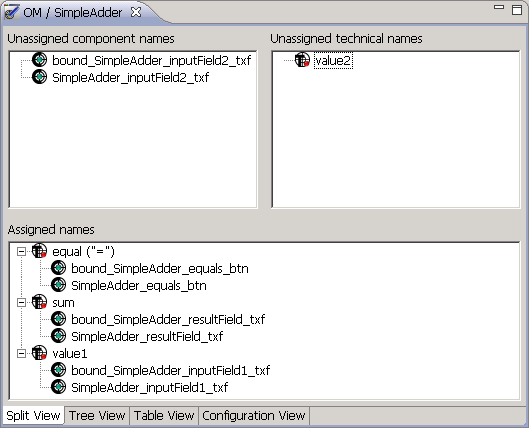
\includegraphics[width=\bxpicwidth]{Tasks/Objectmapping/PS/objectmappinghowto}
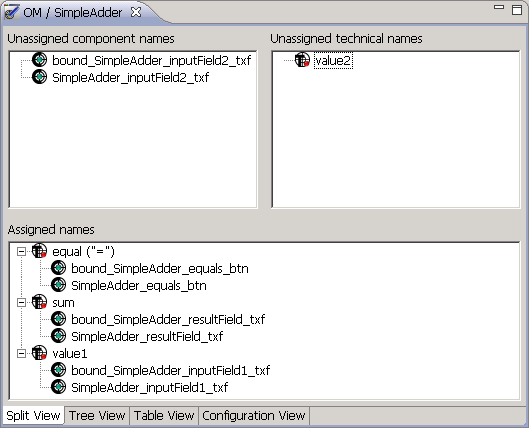
\includegraphics{Tasks/Objectmapping/PS/objectmappinghowto}
\caption{Object Mapping Editor}
\label{objectmappingeditor}
\end{center}
\end{figure}

\begin{figure} [h]
\begin{center}
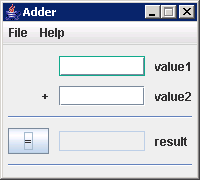
\includegraphics{Tasks/Objectmapping/PS/greenborders}
\caption{Green Border around Supported Component}
\label{greenborders}
\end{center}
\end{figure}


